\chapter{QoS sztohasztikus becslése}
A diplomaterv feladatai közé tartozik a Quality of Service (QoS), azaz a szolgáltatás minőségének a biztosításának megvalósítása, továbbá az 5G feltételrendszerével a feladat áttekintése.
\begin{figure}
	\centering
	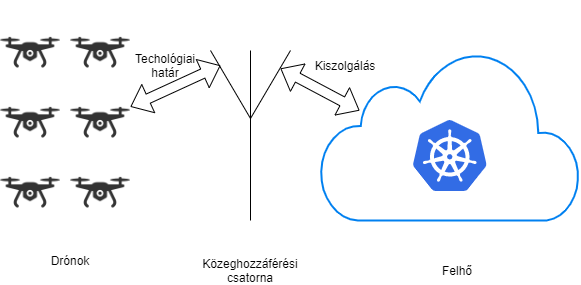
\includegraphics[width=\linewidth]{figures/qos.png}
	\caption{Több robot kiszolgálásának felhőből a durva modellje}
	\label{fig:qos}
\end{figure}
Egy durva modellben (\ref{fig:qos}. ábrán látható), a robotok felhővel való kiszolgálásának késleltetését két helyen vizsgálhatjuk:
\begin{enumerate}
\item Van egy technológiai határ, amit a nagy eszközszám kommunikációja határoz meg, ez annak a határa, hogy hány eszköz tud stabilan kommunikálni egy hálózaton, például az egyetem hálózatán. Tudjuk, hogy a Bluetooth, IEEE 802.11 különböző változatai és az LTE is más-más eszközmennyiséget tud kiszolgálni egyszerre egy antennán keresztül. Ebben a fejezetben ennek a limitációnak a kibővétéséről nem fog szó esni, de későbbiekben megnézzük, hogy mit tehet ennek a kibővítésnek az érdekében az 5G technológia.
\item A másik a felhő kihasználtsága és feladatelvégzési ideje. Itt a felhő feladatokat kap sorban valamilyen intenzitással és ezeknek a feladatoknak van egy elvégzési ideje, nyilván a Kubernetes cluster kapacitásának függvényében. Nyilvánvaló, hogy a felhő kihasználtsága valamilyen függőségben lesz a kiszolgálás idejével, ami a QoS-t meghatározza. Ebben a fejezetben azt a határt nézzük meg, hogy hogyan tudjuk méretezni a felhőnket, hogy valamilyen $t_0$ felsőbecsléssel élhessünk egy drón kiszolgálásának idejére, természetesen miliszecundumban.
\end{enumerate}

\section{Tömegkiszolgálási modell}
Valamennyi $R$ drón valamilyen $\lambda$ [kérés/s] intenzitással fordul a felhőhöz, hogy az számítást végezzen a kameraképen és megmondja mit kell csinálni. Erre a drón valamennyi idő múlva választ kap és ennek az időnek nem szabad elszállni. A megbecsléséhez majd meg kell mérnünk, hogy átlagosan egy ilyen kérést a felhő mennyi idő alatt végez el, ez legyen $\mu$.
Feltételezhetjük, hogy nagy $R$ drónszám esetén függetlenül érkeznek a kérések, így modellezhetünk Poission folyamattal a beérkező kéréseket nézve. Tehát ha egy drónnak a kérési intenzitása valamilyen feladatra $\frac{\lambda}{R}$, akkor az összes drónnak $\lambda$.
Ezt tekinthetjük egy Markov folyamatnak, ahol az infinitezimális generátorból tudunk majd valamilyen sorhossz várhatóértékeket kiszámítani. Mivel nem vesznek el kérések, csupán torlódik a sor, ezért ez egy M/M/1 kiszolgálási modell. \cite{toki}
Az infinitezimális generátor definíció szerint
\[ G =
\begin{bmatrix}
-\lambda & \lambda & 0 & 0 & 0 & 0 & ... \\
\mu & -(\lambda+\mu) & \lambda & 0 & 0 & 0 & ... \\
0 & \mu & -(\lambda+\mu) & \lambda & 0 & 0 & ... \\
0 & 0 & \mu & -(\lambda+\mu) & \lambda & 0 & ... \\
0 & 0 & 0 & \mu & -(\lambda+\mu) & \lambda & ... \\
: & : & : & : & : & : & .
\end{bmatrix}
\]
Ami annyit mond, hogy a várakozó eszközök sorhossza $\lambda$ intenzitással növekedik egyet, amikor érkezik egy kérés és $\mu$ intenzitással csökken egyet, amikor elvégződik egy kérés.

\section{Várakozási idő várható értéke}
Ha a tömegkiszolgálási modellünk jó és tényleg tekinthetjük a kérések eloszlását egy véletlennek, amit nem nagyon specifikus drónirányítás esetben megtehetünk, akkor egy M/M/1-es rendszer kiszolgálási késleltetését kell megnéznünk. A \cite{toki} jegyzet 4.4-es fejezet bebizonyítja,ennek a modellnek a késleltetését, ami a drón kérésére visszakapott válasz a felhő és az antenna között a $D$ késleltetéssel arányos. A jegyzet bizonyítása alapján: \[ D = \frac{1}{\mu - \lambda} \]
